\subsection{Tensors \hfill(Release 1/2017)}\label{subsec:Tensors}

Tensors are mathematical objects that define relationships between scalars, vectors, matrices, and other tensors. Tensors are represented as \textit{arrays} of various dimensionality (defined by rank or order). The moniker ``tensor'' in general suggests a higher-rank array (most often $\geq$3 dimensions), but scalars, vectors, and matrices are also tensors.

In the MSE graduate core, students will encounter tensors of various rank. In physical science, tensors characterize the properties of a physical system. Tensors are the \textit{de facto} tool used to describe, for example, diffusion, nucleation and growth, states of stress and strain, Hamiltonians in quantum mechanics, and many, many, more physical phenomenon. Physical processes of interest to Materials Scientists take place in Euclidean 3-space (${\rm I\!R}^3$) are are well-described by tensor representations.

We build up our description of the handling of tensors starting by separately describing rank-0, rank-1, rank-2, and rank-3 tensors. Tensors of lower ranks should be familiar --- students will have encountered them previously as scalars (rank-0), vectors (rank-1), and matrices (rank-2). The term \emph{tensors} typically denotes arrays of higher dimensionality (rank $\geq3$). Physical examples include the rank-2 \href{https://en.wikipedia.org/wiki/Cauchy_stress_tensor}{Cauchy stress tensor} which describes the stress state of a at a point within a material), the rank-3 piezoelectric tensor (which relates the dielectric polarization of a material to a stress state), and the rank-4 stiffness tensor (which relates strain state and stress state in a system that obeying Hooke's law).

Classifications of tensors by  rank allows us to quickly identify the number of tensor components we will work with: a tensor of order $p$ has $N^p$ components, where $N$ is the dimensionality of space in which we are operating. In general, you will be operating in Eucledian 3-space, so the number of components of a tensor is defined as $3^p$. 

\paragraph{Scalars}are considered tensors with \emph{order} or \emph{rank} of 0. Scalars represent physical quantities (often accompanied by a unit of measurement) that possess only a magnitude: e.g., temperature, mass, charge, and distance. Scalars are typically represented by Latin or Greek symbols and have $3^{0} = 1$ component.

\paragraph{Vectors}are tensors with a \emph{rank} of 1. In symbolic notation, vectors are typically represented using lowercase bold or bold-italic symbols such as $\mathbf{u}$ or $\pmb{a}$. Bold typeface is not always amenable to handwriting, however, and so the a right arrow accent is employed: $\vec{u}$ or $\vec{a}$.  Students are likely to encounter various conventions depending on their field of study.

In ${\rm I\!R}^3$ a vector is defined by $3^{1} = 3$ components. In \textit{xyz} Cartesian coordinates we utilize the Cartesian basis with 3 orthogonal unit vectors $\{\mathbf{e}_{\mathbf{x}}\text{, } \mathbf{e}_{\mathbf{y}}\text{, } \mathbf{e}_{\mathbf{z}}\}$. We define 3D vector $\mathbf{u}$ in this basis with the components ($u_x$, $u_y$, $u_z$), or equivalently  ($u_1$, $u_2$, $u_3$). Often, we represent the vector $\mathbf{u}$ using the shorthand $u_i$, where the $i$ subscript denotes an index that ranges over the dimensionality of the system (1,2,3 for ${\rm I\!R}^3$, 1,2 for ${\rm I\!R}^2$). %Need to figure out \bm!

Vectors are often encountered in a bracketed vertical list to facilitate matrix operations. Using some of the notation defined above:

\begin{equation}
\mathbf{u} = u_i = 
	\begin{bmatrix}
    u_x \\
    u_y \\
    u_z
	\end{bmatrix} =
	\begin{bmatrix}
    u_1 \\
    u_2 \\
    u_3
	\end{bmatrix}
	\label{eq:Vector}
\end{equation}

\paragraph{Matrices}are tensors with a \emph{rank} of 2.  In ${\rm I\!R}^2$ a matrix has $2^{2} = 4$ components and in ${\rm I\!R}^3$ a matrix has $3^{2} = 9$ components. As with vectors, we will use the range convention when denoting a matrix, which now possesses two subscripts, $i$ and $j$. We use the example of the true stress, or \href{https://en.wikipedia.org/wiki/Cauchy_stress_tensor}{Cauchy stress tensor}, $\sigma_{ij}$:

\begin{equation}
\sigma_{ij} =  
	\begin{bmatrix}
    \sigma_{xx} & \sigma_{xy} & \sigma_{xz}\\
    \sigma_{yx} & \sigma_{yy} & \sigma_{yz}\\
    \sigma_{zx} & \sigma_{zy} & \sigma_{zz}\\
	\end{bmatrix}
\end{equation}

Where the diagonal represents the normal components of stress and the off-diagonal represents the shear components of the stress. In this notation the first index denotes the row while the second denotes the column ($x = 1$, $y = 2$, $z = 3$).

\paragraph{Tensors} A rank-3 tensor in ${\rm I\!R}^3$ has $3^{3} = 27$ components and is represented in range notation using subscripts $i$, $j$, and $k$, e.g., $T_{ijk}$ . At rank-3 (and it is even worse in rank-4, requiring an array of rank-3 tensors) it begins to become difficult to represent clearly on paper. An example of a simple tensor --- \href{https://en.wikipedia.org/wiki/Levi-Civita_symbol#Three_dimensions_2}{the rank-3 permutation tensor} --- is shown in Fig. \ref{fig:PermutationTensor}. You can also watch \href{https://www.youtube.com/watch?v=f5liqUk0ZTw}{this video} which helps with the visualization. 

\begin{figure}%
	\centering
	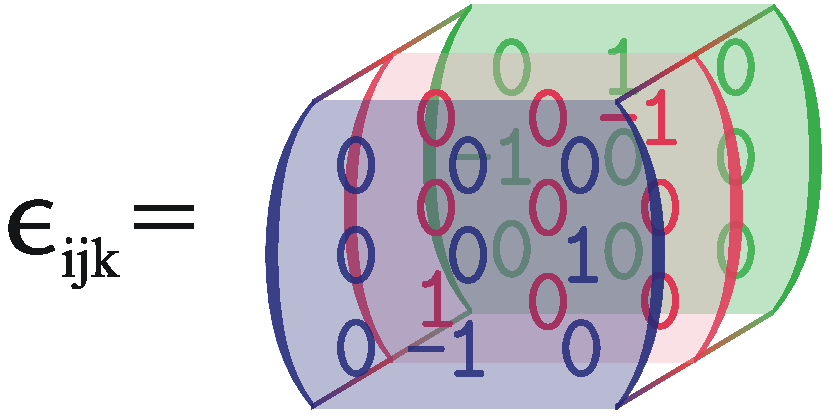
\includegraphics[scale=0.5]{PermutationTensor}%
	\caption{The rank-3 permutation tensor, by Arian Kriesch. corrections made by Xmaster1123 and Luxo (Own work) [GFDL (http://www.gnu.org/copyleft/fdl.html), CC-BY-SA-3.0 (http://creativecommons.org/licenses/by-sa/3.0/)}%
	\label{fig:PermutationTensor}%
\end{figure}

One can write the $i = 1,2,3$ matrices that stack to form this tensor as: %This should be replaced as just a general tensor. I can adapt the tensor.

\begin{equation}
	\epsilon_{1jk}=
	\begin{bmatrix}
		0 & 0 & 0\\
		0 & 0 & 1\\
		0 & -1 & 0
	\end{bmatrix}
\end{equation}

\begin{equation}
	\epsilon_{2jk}=
	\begin{bmatrix}
		0 & 0 & -1\\
		0 & 0 & 0\\
		1 & 0 & 0
	\end{bmatrix}
\end{equation}

\begin{equation}
	\epsilon_{3jk}=
	\begin{bmatrix}
		0 & 1 & 0\\
		-1 & 0 & 0\\
		0 & 0 & 0
	\end{bmatrix}
\end{equation}




	%\subsubsection{Vector Calculus \hfill(Release TBD)}
	%
	%\textit{\textbf{Encountered in: MAT\texttt{\_}SCI 406, 408}} 